\section{Method}

The MultiGWAS tool has three main steps: the adjustment stage, the multi analysis stage, and the integration stage (Fig. \ref{pipeline}). In the first stage, MultiGWAS processes the configuration file. Then it cleans and filters the genotype and phenotype, and  MultiGWAS "diploidize" the genomic data. In the second stage, each GWAS tool runs in parallel. In the last stage, after the output files scanning, a summary of results is generated in a report that contains score tables, Venn diagrams, SNP profiles, and Manhattan plots. 

\begin{figure}
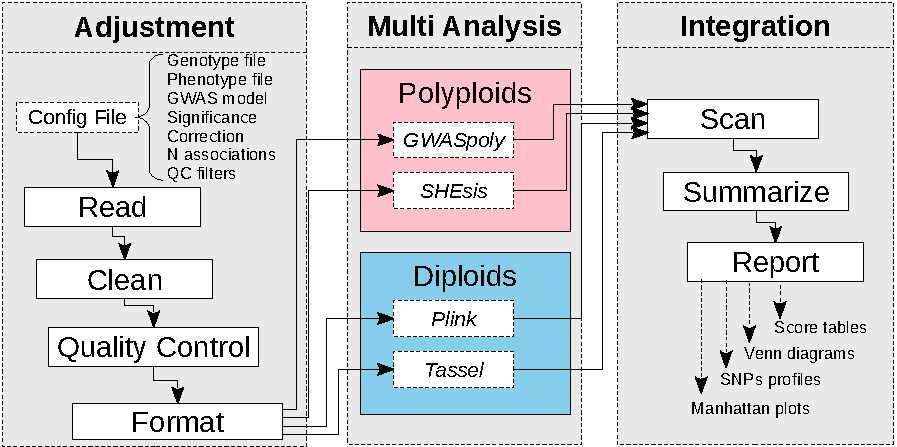
\includegraphics[width=12cm]{images/multi-gwas-flowchart-horizontal-stages-config.pdf}
\caption{MultiGWAS flowchart has three stages: adjustment, multi analysis, and integration.\label{pipeline}}

\end{figure}

\subsection{Adjustment stage} 
MultiGWAS takes as input a configuration file where the user specifies the genomics data along with the parameters that will be used by the four tools. Once the configuration file is processed, MultiGWAS preprocess the data that is cleaning, filtering, and checking data quality. The output of this stage corresponds to the inputs for the four programs at the Multi Analysis stage.


%genotype/phenotype filenames, genome-wide significance threshold, multiple testing correction methods, GWAS model, number of associations to be reported, and TRUE or FALSE whether to use quality control (QC) filters or not. 
 
\subsubsection{Configuration file}
The configuration file includes the following settings that we briefly describe:% (1) Input genotype and phenotype file names (2) GWAS model, (3) Significance threshold, (4) Correction (5) Quality Control (QC) filters and (6) number of associations to report. 

\paragraph{Input genotype and phenotype files:}
Currently, MultiGWAS uses two input files, one for genotype and the other for the phenotype. Both data correspond to data matrices with column and row names (Figure \ref{fig:File-Formats}). The genotype file uses SNP markers in rows and samples in columns (Figure \ref{fig:File-Formats}a). The phenotype file uses samples in rows and traits in columns (Figure \ref{fig:File-Formats}b) with the first column corresponding to the sample name and the second column to trait value.

%Paula: Luis una pregunta, recibimos solo formato ACGT? o recibimos otro formato?? 
% R/ Actualmente solo formato GWASpoly (dos archivos), se podría facilmente formato númerido, dos archivos (ClusterCall) con o sin info de mapa (CHROM, POSITION), y tal vez formato PLINK (tres archivos).

\begin{figure}[H]
\begin{centering}
\begin{minipage}[t]{0.6\columnwidth}%
\begin{center}
\fbox{\begin{minipage}[t]{0.99\columnwidth}%

\scriptsize\textcolor{gray}{\texttt{Marker,Chrom,Pos,Indiv01,Indiv02,Indiv03,...}}
\texttt{c2\_41437,0,805179,AAAG,AAGG,AAGG,...}
\texttt{c2\_24258,0,1252430,AAGG,AGGG,GGGG,...}
\texttt{c2\_21332,0,3499519,TTCC,TTCC,TTCC,... }\\
\texttt{...}%
\end{minipage}}\\
a
\par\end{center}%
\end{minipage}~~~~~~~~~%
\begin{minipage}[t]{0.3\columnwidth}%
\begin{center}
\fbox{\begin{minipage}[t]{0.99\columnwidth}%
\scriptsize\textcolor{gray}{\texttt{Individual,Traitname}}

\texttt{Indiv01, 3.59}\\
\texttt{Indiv02, 4.07}\\
\texttt{Indiv03, 1.05}

\texttt{...}%
\end{minipage}}\\
b
\par\end{center}%
\end{minipage}
\par\end{centering}
\begin{centering}
\par\end{centering}
\caption{\textbf{MultiGWAS genotype and phenotype formats}. Both files are in CSV format (Comma Separated Values) and contain as first row the header labels of the columns. Although the header labels are arbitrary, the column order is obligatory. \textbf{a.} Genotype file format, where ``Marker'', ``Chrom'', and ``Pos'', correspond to the names for marker name, chromosome, and position in the first three columns respectively. The next columns correspond to the columns for the samples content. \textbf{b.} Phenotype file format, where ``Individual'' and ``Traitname'' are the column names for the individual and trait names, respectively.\label{fig:File-Formats}}
\end{figure}

\paragraph{GWAS model:}
MultiGWAS implements two types of GWAS analysis: (1) \textit{naive} and (2) \textit{full}. The \textit{naive} model without any control for structure or relatedness between samples (without any additional parameters). Whereas the \textit{full model}, known as the Q+K model, takes into account population structure (Q) and relatedness (K) to prevent false associations. We estimate Q and K inside MultiGWAS. 

Both models use linear regression. The \emph{naive} is modeled with Generalised Linear Models (GLMs, Phenotype + Genotype), and the \emph{full} is modeled with Mixed Linear Models (MLMs, Phenotype + Genotype + Structure + Kinship). The default model used by MultiGWAS is the \emph{full model} (Q+K) \cite{Yu2006}, which is described with the following equation:

\[
y=X\beta+S\alpha+Q\nu+Z\mu+e
\]

where $y$ is the vector of observed phenotypes; $\beta$ is a vector of fixed effects; $\alpha$ is a vector of SNP effects; $\nu$ is a vector of population effects; $\mu$ is a vector of polygene background effects; $e$ is a vector of residual effects; $Q$, modeled as a fixed effect, refers to the incidence matrix for subpopulation covariates relating $y$ to $\nu$; and $X$, $S$ and $Z$ are incidence matrices of ones and zeros relating $y$ to $\beta$, $\alpha$ and $\mu$, respectively.

%Paula: QUantitavie trait nucleotides??? duda del termino
%Luis R/ No se en realidad que es, coloqué la formula pq se necesitaba algo formal,y esta es la más simple y menos extensa que encontré.


% Este parrafo va a cambiar un poco pq la corrección se hace solo al nivel de significancia y no a los p-values, así lo hace GWASpoly y así lo recomiendan en foros de GWAS, pero tengo que sutentarlo.
\paragraph{Genome-wide significance and multiple testing correction:}
GWAS searches SNPs associated with the phenotype in a statistically significant manner. A threshold or significance level $\alpha$ is specified and compared with the \emph{p-value} derived for each association score. Standard significance levels are 0.01 or 0.05 \cite{Gumpinger2018,Rosyara2016}.  However, due to the massive number of statistical tests performed by GWAS, the \emph{p-values} must be adjusted appropriately, performing a correction method for multiple hypothesis testing (MHT). 

MultiGWAS allows two MHT methods for adjusting \emph{p-values}: the Bonferroni correction and the false discovery rate (FDR). In the case of the Bonferroni correction, the threshold is $\alpha/m$, where \emph{m }is the number of valid markers from the genotype matrix (not missing or null values). (default $\alpha$=0.05, Correction=Bonferroni)

%Paula: Luis estos parámetro por default de QC y alpha faltan
\paragraph{Quality Control:}

A control step is necessary to check the input data for genotype or phenotype errors or poor quality that can lead to spurious GWAS results. MultiGWAS uses the following filters to control the data quality: Minor Allele Frequency (MAF), individual missing rate (MIND), SNP missing rate (GENO), and Hardy\-Weinberg threshold (HWE). 

MAF of \{x\} filters out SNPs with minor allele frequency below \{x\} (default 0.01); MIND of \{x\} filters out all individuals with missing genotypes exceeding \{x\}{*}100\% (default 0.1); GENO \{x\} filters out SNPs with missing values exceeding \{x\}{*}100\% (default 0.1); and HWE filters out SNPs which have Hardy-Weinberg equilibrium exact test \emph{p-value} below the \{x\} threshold.

MultiGWAS does the MAF filtering. We use the PLINK package \cite{Gumpinger2018} for the other three filters: MIND, GENO, and HWE. Once we have the samples and SNPs that pass the filters, then we generate an input file for each package used. 

\paragraph{Number of best ranked associations:}
Criticism has arisen in considering only statistically significant associations as the only possible correct associations \cite{Thomson2011,Kaler2019}. Many of low \emph{p-value} associations, closer to being significant, are discarded due to the stringent significance levels, and consequently increasing the number of false negatives. To help to analyze both significant and non-significant associations, MultiGWAS provides the option to specify the number of best-ranked associations, adding the corresponding  \emph{p-value} to each association found.  In this way, it is possible to enlarge the number of results, and we can observe replicability in the results for different programs. Nevertheless, we present each association with the corresponding \emph{p-value}.%  We present the resultant associations in different tables and graphics reported by MultiGWAS (see Figure \ref{fig:-View-Shared-SNPs}). 




\subsubsection{Data preprocessing}
Once the configuration file is processed, the genomic data is read and cleaned by selecting individuals present in both genotype and phenotype and excluding individuals and SNPs that have poor quality. MultiGWAS applies four quality control filters commonly used in GWAS analysis

At this point, the format   "ACGT" suitable for the polyploid software GWASpoly and SHEsis, is "diploidized" for PLINK and TASSEL. The homozygous tetraploid genotypes are converted to diploid thus: (e.g.,AAAA\textrightarrow AA, CCCC\textrightarrow CC, GGGG\textrightarrow GG,
TTTT\textrightarrow TT). Moreover, for tetraploid heterozygous genotypes, the conversion depends on the reference and alternate alleles calculated for each position (e.g., AAAT\textrightarrow AT,
... ,CCCG\textrightarrow CG). After this process, MultiGWAS transform the genomic data into the formats required for each software.



\subsection{Multi analysis stage} 

%\subsubsection{Tools}
We have selected four GWAS software tools to be integrated into our multiGWAS tool. Two designed specifically for polyploid species: GWASpoly \cite{Rosyara2016} and SHEsis \cite{Yong2006}. Another two designed for diploids species and extensively used in humans and plants: PLINK \cite{Purcell2007,Chang2015} and TASSEL \cite{Bradbury2007}, respectively.  At this stage, MultiGWAS runs the four packages simultaneously. We briefly describe each package as follows.

%MultiGWAS runs in parallel using two types of statistical models specified in the parameters file, the Full model (Q+K) and Naive (i.e., without any control) \cite{Sharma2018}. The Full model (Q+K) controls for both population structure and individual relatedness. For population structure, MultiGWAS uses the Principal Component Analysis (PCA) and takes the top ten PC as covariates. For relatedness, the tool uses kinship matrices that TASSEL and GWASpoly calculated separately, and for PLINK and SHEsis depends on the King software \cite{Manichaikul2010}. 

As MultiGWAS implements two types of GWAS analysis,  \emph{naive} and  \emph{full}, each tool is called in two different ways.
%The naive without any additional parameter, but the full with two parameters that take into account for population structure (Q) and relatedness (K) to prevent false associations.

\subsubsection{GWASpoly}

GWASpoly \cite{Rosyara2016} is an R package designed for GWAS in polyploid species used in several studies in plants \cite{Berdugo2017,Ferrao2018,Sharma2018,Yuan2019}. GWASpoly uses a Q+K linear mixed model with biallelic SNPs that account for population structure and relatedness. Also, to calculate the SNP effect for each genotypic class, GWASpoly provides a general gene action model along with four additional models: additive, simplex dominant, and duplex dominant. We use all the models to find associations. % Threshold for each model

MultiGWAS is using GWASpoly version 1.3. The population structure and relatedness, used in the \emph{full} model, are estimated using the first five principal components and the kinship matrix, respectively, both calculated with the algorithms built-in GWASpoly.  


\subsubsection{SHEsis}

SHEsis \cite{Shen2016} is a program written in C designed for polyploid species. It includes single locus association analysis, among others. It is based on a linear regression model, and it has been used in some studies of animals and humans \cite{Qiao2015,Meng2019}. 

MultiGWAS is using version 1.0, which does not take account for population structure or relatedness. However, MultiGWAS externally estimates relatedness for SHEsis by excluding individuals with cryptic first-degree relatedness using the algorithm implemented in PLINK 2.0 (see below).


\subsubsection{PLINK}

PLINK \cite{Purcell2007} is a program written in C frequently used in diploids species in particular humans \cite{Power2016}. PLINK includes univariate GWAS using two-sample tests and linear regression models.

MultiGWAS is using two versions of PLINK: 1.9 and 2.0. We use the linear regression from PLINK 1.9 to achieve both types of analysis, \emph{naive} and \emph{full}. We use the first five principal components calculated with the PLINK 1.9 built-in algorithm to estimate the population structure. We estimate the relatedness from the kinship coefficients calculated with the PLINK 2.0 built-in algorithm, removing the close relatives or individuals with the first-degree relatedness.

\subsubsection{TASSEL}

TASSEL  \cite{Bradbury2007}  is a GWAS program written in Java, frequently used for diploid plant studies. TASSEL was developed for maize data \cite{Alvarez2017,Zhang2018}. For association analysis, TASSEL includes the general linear model (GLM) and mixed linear model (MLM) that accounts for population structure and relatedness.

MultiGWAS is using TASSEL 5.0. The \emph{naive} GWAS uses GLM. The \emph{full} GWAS uses MLM with two parameters: one for population structure, using the first five principal components, and another for relatedness, using the kinship matrix with centered IBS method, both calculated with the TASSEL built-in algorithms.


\subsection{Integration stage.} The outputs resulting from the four software are scanned and processed to identify both significant and best-ranked associations. MultiGWAS corrects (correction method defined in the configuration file) the p-values and calculates the threshold value for each associated marker. The calculation uses the number of valid genotype calls (i.e., non-missing genotypes, phenotypes, and covariates). 

\begin{figure}

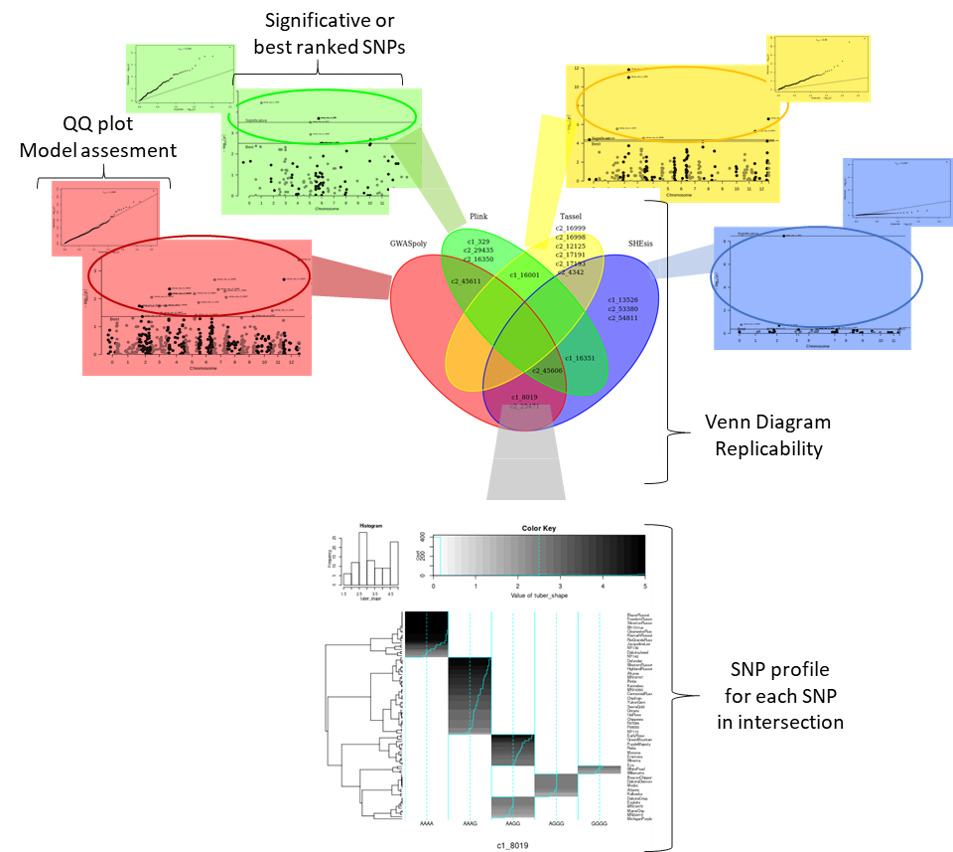
\includegraphics[width=15cm]{images/Reportes_Metodologia.png}
\caption{We present several reports. For each tool, first a QQ plot that asses the resultant p-values.  Second, a Manhattan plot for each tool with two lines, blue and red, respectively, is the lower limit for the best ranked and significative SNPs. We present two Venn diagrams, one for the significative SNPs and one for N best-ranked SNPs of each tool. We show the results for GWAspoly, PLINK, TASSEL, and SHEsis in red, green, yellow, and blue, respectively. Moreover, for each SNP that is in the intersection; thus, that is predicted by more than one tool we provide SNP profile. \label{reports}}
\label{pipeline}
\end{figure}

At this stage, We integrate the results to evaluate reproducible results among tools (Fig \ref{reports}). But, We still report a summary for the results of each tool:
\begin{itemize}
    \item A Quantile-Quantile (QQ) plots for the resultant p-values of each tool and the corresponding degree of inflation $\lambda$ to asses the degree of the test statistic inflation.
    \item AA Manhattan plot of each tool with two lower thresholds, one for the best-ranked SNPs, and another for the significant SNPs. 
\end{itemize}

To present the replicability, we use two sets: (1) the set of all the significative SNPs provided by each tool and (2) the set of all the best-ranked SNPs. For each set, we present a Venn diagram that shows SNPs predicted exclusively by one tool and intersections that help to identify the SNPs predicted by one, two, three, or all the tools. In addition, we provide detailed tables for the two sets.

For each SNP predicted more than once, we provide what we call the SNP profile. That is a heat diagram for a specific SNP, where each column is a genotype state AAAA, AAAB, AABB, ABBBB, BBBBB. And each row corresponds to a sample. Samples with close genotypes form together clusters. Thus to generate the clusters, we do not use the phenotype information. However, we present the phenotype information in the figure as the color. This figure visually provides information regarding genotype and phenotype information simultaneously for the whole population. We present colors as tones between white and black for color blind people. 


MultiGWAS generates a report, one document with the content previously described. Besides, there is a folder with the individual figures just in case the user needs one. In the supplementary information, we include a report and a description of the report content\textcolor{red}{(supplementary information XXX)}

%PAula: infomración suplementary con reporte completo y figuras. Y explicación del reporte

In the following section, we present the results applied to a public dataset. 
